\begin{figure*}[t]
\centering
% Vector drawing generated by tools/figures/build.py; rerun it after changing the figure.
\ifbilingual
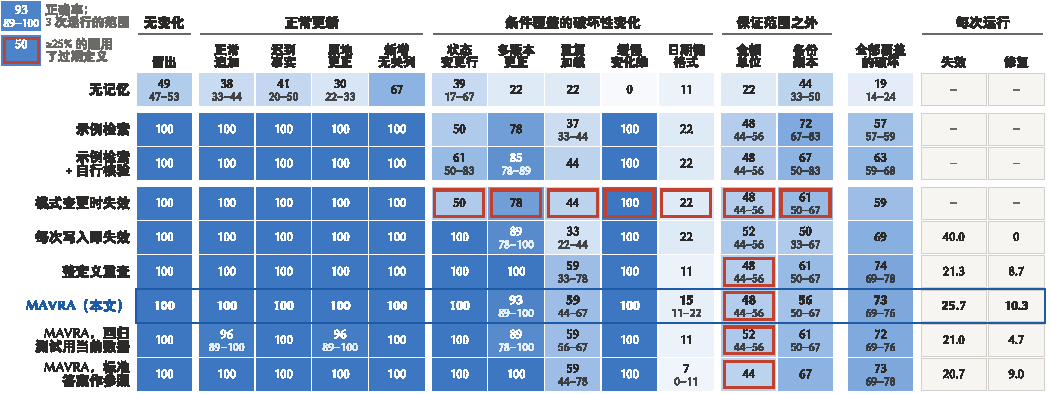
\includegraphics[width=\textwidth]{figures/scenario-changes-zh}
\else
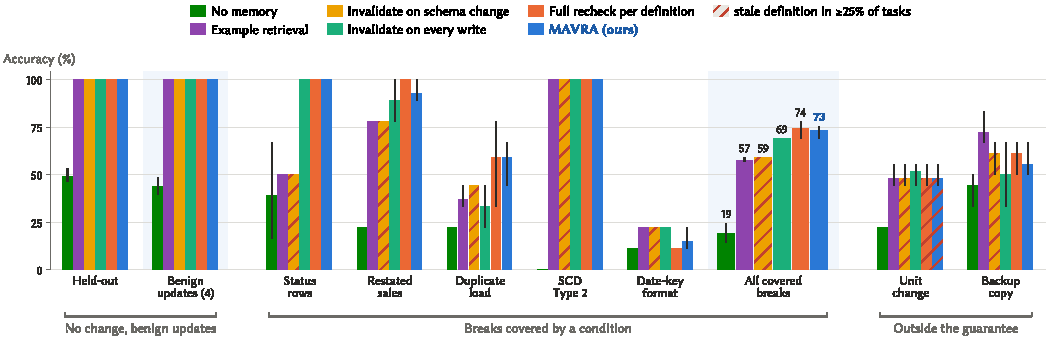
\includegraphics[width=\textwidth]{figures/scenario-changes}
\fi
\caption{\bt{Accuracy of the user agent by data change, DeepSeek V4.1 Flash, for the baselines and \system. Each marker is the accuracy over three independent runs and the line behind it spans the three runs; a red ring marks settings in which at least 25\% of the tasks used a stale definition, i.e., one whose canonical SQL answers that setting's questions incorrectly. Brackets group the changes by the condition they target. Right: invalidations and published repairs per run for the methods that keep definitions, lines spanning the runs; the full recheck and the regression ablation appear only here and in the text. In all, \ScenCells\ runs, \ScenValidTasks\ scored tasks, and \ScenAgentHours\ agent-hours.}{按数据变化划分的用户端智能体正确率，DeepSeek V4.1 Flash，基线与 \system。每个点是 3 次独立运行全部题目上的正确率，点后的细线是 3 次运行的范围；红圈表示该情形下至少 25\% 的题使用了过期定义，即其规范 SQL 在该情形下答错的定义。轴下的括线按变化针对的条件分组。右：维护定义的方法每次运行的失效数与发布的修复数，细线为各次运行的范围；整定义重查与回归测试的消融只出现在这里和正文。共 \ScenCells\ 次运行、\ScenValidTasks\ 道计分题、\ScenAgentHours\ 智能体小时。}}
\label{fig:scenarios}
\Description{Left: a dot plot with the twelve settings on the horizontal axis, grouped by brackets into none, benign, grain, join fan-out, completeness, not covered, and ambiguous fix, and accuracy from 0 to 100 percent on the vertical axis; six methods per setting (no memory, example retrieval, example retrieval with self-verification as diamonds, invalidation on schema change, invalidation on every write, MAVRA), each a marker at the accuracy over runs with a thin line for the range over the three runs. All sharing methods sit at 100 percent on the held-out and benign settings while no memory lies between 30 and 67 percent. Under status-change rows MAVRA and invalidation on every write are at 100 percent, example retrieval and invalidation on schema change at 50, the latter with a red ring, self-verification at 61. Under restatements MAVRA is at 93, every write at 89, example retrieval and schema change at 78 (red ring); under duplicate loads MAVRA at 59, example retrieval at 37, schema change at 44 (red ring), every write at 33. Under SCD Type 2 every sharing method is at 100, schema change ringed. Under the date-key format change all methods lie between 11 and 22 percent, under the unit change between 44 and 52, and under the backup copy example retrieval is highest at 72 with MAVRA at 56. Right: horizontal bars of invalidations (light) and published repairs (solid) per run with the range over runs: invalidation on every write 40 and 0, MAVRA 25.7 and 10.3, full recheck per definition 21.3 and 8.7, MAVRA with the regression test on current data 21.0 and 4.7.}
\end{figure*}
